%%---------------------------------------------------------------------------%%
%% draco-3_0_0.tex
%% Thomas M. Evans
%% $Id$
%%---------------------------------------------------------------------------%%
\documentclass[11pt]{nmemo}
\usepackage[centertags]{amsmath}
\usepackage{amssymb,amsthm,graphicx}
\usepackage[mathcal]{euscript}
\usepackage{tmadd,tmath}
\usepackage{cite}
\usepackage{tabularx}

%%---------------------------------------------------------------------------%%
%% DEFINE SPECIFIC ENVIRONMENTS HERE
%%---------------------------------------------------------------------------%%
%\newcommand{\elfit}{\ensuremath{\operatorname{Im}(-1/\epsilon(\vq,\omega)}}
%\msection{}-->section commands
%\tradem{}  -->add TM subscript to entry
%\ucatm{}   -->add trademark footnote about entry

\newcommand{\draco}{Draco}
\newcommand{\dracor}{\draco-3\_0\_0}
\newcolumntype{L}{>{\ttfamily}X}

\newcommand{\autoconf}{\textsf{Autoconf}}
\newcommand{\automake}{\textsf{Automake}} 
\newcommand{\CVS}{\textsf{CVS}}  
\newcommand{\make}{\textsf{Make}}

%%---------------------------------------------------------------------------%%
%% BEGIN DOCUMENT
%%---------------------------------------------------------------------------%%
\begin{document}

%%---------------------------------------------------------------------------%%
%% OPTIONS FOR NOTE
%%---------------------------------------------------------------------------%%

\toms{Distribution}
%\toms{Joe Sixpak/XTM, MS B226}
\refno{CCS--4:03-18(U)}
\subject{Release of \dracor}

%-------NO CHANGES
\divisionname{Computer and Computational Sciences Division}
\groupname{CCS-4:Transport Methods Group}
\fromms{Thomas M. Evans/CCS-4 D409}
\phone{(505)665--3677}
\originator{tme}
\typist{tme}
\date{6/4/2003}
%-------NO CHANGES

%-------OPTIONS
%\reference{NPB Star Reimbursable Project}
%\thru{P. D. Soran, XTM, MS B226}
%\enc{list}      
%\attachments{list}
%\cy{list}
%\encas
%\attachmentas
%\attachmentsas 
%-------OPTIONS

%%---------------------------------------------------------------------------%%
%% DISTRIBUTION LIST
%%---------------------------------------------------------------------------%%

\distribution {
  CCS--4, MS D409\\
  CCS--2, MS D413\\
}

%%---------------------------------------------------------------------------%%
%% BEGIN NOTE
%%---------------------------------------------------------------------------%%

\opening

\begin{abstract}
  We have released \dracor.  This release contains some significant
  modifications to the Draco Build System.  Additionally, we have
  changed the component tagging policy.  These changes, as well as
  other modifications, are summarized in this release announcement.
\end{abstract}

%%---------------------------------------------------------------------------%%

\section{\draco\ Contributors}

The following people are contributors to \draco:
\begin{center}
  \begin{tabular}{ll}
    Tom Evans & \texttt{tme@lanl.gov} \\
    Kelly Thompson & \texttt{kellyt@lanl.gov} \\
    Todd Urbatsch & \texttt{tmonster@lanl.gov} \\
    Kent Budge & \texttt{kgbudge@lanl.gov} \\
    Mike Buksas & \texttt{mwbuksas@lanl.gov} \\
    Jim Warsa & \texttt{warsa@lanl.gov} \\
    Rob Lowrie & \texttt{lowrie@lanl.gov} \\
    Todd Adams & \texttt{bta@lanl.gov} \\
  \end{tabular}
\end{center}

%%---------------------------------------------------------------------------%%

\section{New Policies}

\draco\ is the CCS--4 Transport Components library~\cite{rn98046}.
\draco\ releases up to \draco-2\_4\_0 have been somewhat informal,
but, nonetheless, they have followed the policies laid down in
Ref.~\cite{xtm:9936}.  With \dracor\ we are embarking upon a more
proactive policy of release documentation.  In addition to tagging and
testing code as specified in Ref.~\cite{xtm:9936}, we will now
accompany each major-number release with a (small) memorandum
announcing the release.

Each \draco\ release is documented in the \texttt{draco/ChangeLog}
file.  This policy remains unchanged.

We are making a minor change to the release procedures\footnote{We
  dropped the \texttt{last\_stable} tagging mechanism in
  \draco-1\_0\_0.}.  The \textit{Draco Release Policy and
  Procedures}~\cite{xtm:9936} specify that each component package must
have a release tag that is synchronized with a \draco\ release tag.
We are modifying this requirement as follows:
\begin{quote}
  Component package tags should only be used to represent interim
  releases of a component.
\end{quote}
Thus, the \draco\ tag will become the standard version identifier for
each component.  A component may be tagged between \draco\ releases.
In practical terms this means that the \draco\ tag will determine
package releases in most cases.  Component tags should only be used
for interim releases when a new version of a component package is
needed to release client code.  

A new version of \textit{Draco Release Policy and Procedures} will be
released that will explain these changes in more detail.

%%---------------------------------------------------------------------------%%

\section{Draco Component Packages}

\dracor\ contains the following component packages:
\begin{center}
  \begin{tabularx}{\linewidth}{
      >{\setlength{\hsize}{.5\hsize}}L %
      >{\setlength{\hsize}{1.5\hsize}}X}    
    \hline\hline 

    c4 & communication library \\
    cdi & Common Data Interface (CDI) component \\
    cdi\_analytic & CDI analytic data component \\
    cdi\_eospac & CDI EOSPAC wrapper \\
    cdi\_gandolf & CDI GANDOLF wrapper \\
    ds++ & data structures library \\
    imc & Implicit Monte Carlo physics component \\ 
    lapack\_wrap & wrapper to BLAS and LAPACK \\
    mc & Monte Carlo physics component \\
    meshReaders & mesh reader interface \\
    meshReaders\_Services & services for mesh readers (connectivity,
    etc) \\ 
    pcgWrap & wrapper for PCGLIB \\
    plot2D & 2-D plotter interface built on XMGRACE \\
    quadrature & quadrature component \\
    rng & random number generators and SPRNG wrappers \\
    RTT\_Format\_Reader & \texttt{meshReaders} implementation for RTT
    format meshes \\
    stdheaders & C-standard libraries wrapped in the \texttt{std::}
    namespace \\ 
    timestep & a timestep controller component \\
    traits & traits used by other \draco\ components \\
    units & a physics units component \\
    viz & interfaces to visualization tools (EnSight)\\
    xm & glommable expression templates \\  

    \hline\hline 
  \end{tabularx}
\end{center}
There are no inter/intra-component cyclic dependencies in \draco.  The
levelized graph for \draco\ components is shown in
Fig.~\ref{fig:level}.
\begin{figure}
  \label{fig:level}
  \centerline{
    \includegraphics[height=5.5in]{level-3_0_0.ps}}
  \caption{\dracor\ levelized component graph.  Dotted lines signify
    that the dependency if only required for testing.}
\end{figure}

Lines-of-Code (LOC) statistics for the component packages in \dracor\ 
are shown in Fig.~\ref{fig:stats}.  The aggregate LOC statistics for
\dracor\ are:
\begin{center}
  \begin{tabular}{|l|l|} \hline
    Total component package source code & 16963 \\
    Total unit test code & 20153 \\
    Total DBC statements & 1876 \\
    Total comments & 36556 \\
    \hline
  \end{tabular}
\end{center}
\begin{figure}
  \label{fig:stats}
  \centerline{
    \includegraphics[width=6in]{loc-3_0_0.eps}}
  \caption{LOC statistics for \dracor\ component packages.}
\end{figure}

LOC metrics are now stored in \draco\ in
\texttt{draco/doc/code\_stats}.  These metrics will be updated
regularly during major \draco\ releases.

%%---------------------------------------------------------------------------%%

\section{Draco Build System}

There have been considerable changes in the internal implementation of
the Draco Build System (DBS).  These changes were required because of
the changes in \autoconf\ between 2.13 and 2.5+.  For \draco\ users
and clients, these changes can be summarized as follows:
\begin{itemize}
  
\item Each directory now has its own \texttt{aclocal.m4}, generated by
  \automake, and \texttt{configure}, generated by \autoconf.  Both of
  these files are now stored in the \CVS\ repository.
  
\item The \texttt{configure.in} files have been replaced by
  \texttt{configure.ac} files to match the \autoconf\ manual spec.
  The content of these files---aside from some small syntax
  changes---remains unchanged.
  
\item We updated some DBS \autoconf\ macros, particularly those that
  determined the word-sizes.  Vendor macro variable definitions are
  now defined in the macro \texttt{AC\_VENDOR\_DEFINES}.  This macro
  is called at the end of \texttt{AC\_DRACO\_ENV}.
  
\item We added all the variable substitutions to the
  \texttt{AC\_DBS\_VAR\_SUBSTITUTIONS} macro.  As above, this macro is
  called at the end of \texttt{AC\_DRACO\_ENV}.
  
\item \make\ no longer automatically checks the configure system as a
  dependency.  We have provided \make\ targets to do these operations
  explicitly: 
\begin{verbatim}
  gmake configure
  gmake reconfigure
\end{verbatim}
  The \texttt{configure} target will rebuild \texttt{aclocal.m4} and
  \texttt{configure} in the source directory.  It will then
  reconfigure the target directory.  The \texttt{reconfigure} target
  simply reconfigures the target directory without rebuilding
  \texttt{configure} in the source directory.
  
\item The \texttt{draco\_config} script effectively replaces
  \texttt{autoreconf} (\autoconf\ 2.13) for building configure
  infrastructure in the \draco\ source directory.

\end{itemize}
Most of these changes will have little to no impact on \draco\ users
and clients.  

The DBS also has some new features.  These are:
\begin{enumerate}
\item Support for the \textsf{Intel ICC} compiler.
\item Support for IBM PowerPC systems (ASCI White).
\item Support for the IBM \textsf{Visual Age xlC} compiler.
\item New vendors including:
  \begin{itemize}
  \item Trilinos solver package,
  \item Aztec solver package,
  \item GNU Scientific Library GSL.
  \end{itemize}
\end{enumerate}

A new DBS overview document, \textit{The Draco Build System}, is
forthcoming.  However, to keep abreast of regular changes in the DBS,
including new vendors and options, the \textit{Draco Build System}
\textsf{Doxygen} \cite{doxygen} page should be perused.  Regular
changes to the DBS will be updated through \textsf{Doxygen}.  The
released \textit{The Draco Build System} document will provide an
overview.

%%---------------------------------------------------------------------------%%

\section{Draco Tools}

There are several tools of note in \texttt{draco/tools} that have not
been formally documented.  A brief summary of these tools is provided
in Table~\ref{tab:tools}.
\begin{table}
  \caption{Summary of \draco\ tools in \texttt{draco/tools}.}
  \label{tab:tools}
  \begin{center}
    \begin{tabularx}{\linewidth}{
        >{\setlength{\hsize}{.5\hsize}}L %
        >{\setlength{\hsize}{1.5\hsize}}X}
      \hline\hline
      
      build\_ccs4\_release & Script that builds \draco\ releases on
      the CCS Linux LAN \\

      check\_coverage & Script that runs \textsf{gcov} analysis; this
      tool is installed in \texttt{\$prefix/bin}. \\

      count\_loc.sh & Does LOC analysis in a source directory. \\

      draco & Gives information about the \draco\ version and
      configure options; this tool is installed in
      \texttt{\$prefix/bin}. \\

      find\_tags\_diff.py & \textsf{Python} tool that finds the files
      that have been changed since the last component package tag; it
      also prints out the differences in changed files. \\
      
      find\_tags.py & \textsf{Python} tool that finds the files
      that have been changed since the last component package tag. \\

      include\_tree.py & \textsf{Python} tool that builds a levelized
      graph of the component package using \textsf{Dot}. \\

      package\_depends.py & \textsf{Python} tool that shows the
      external \draco\ dependencies for a component package. \\

      regression\_filter.py & \textsf{Python} tool that can be used to
      pipe the results of \texttt{gmake check}; it produces a succinct
      report of the results of all tests. \\

      \hline\hline
    \end{tabularx}
  \end{center}
\end{table}

We have provided a new script, \texttt{draco/get\_tex}.  This script
checks out \LaTeX\ classes from the \CVS\ repository and places them
in the directory \texttt{draco/doc/tex}.  These \LaTeX\ classes may be
needed to build \draco\ documents on remote systems.

%%---------------------------------------------------------------------------%%

\bibliographystyle{rnote}
\bibliography{../../environment/bibfiles/draco}
 
\closing
\end{document}

%%---------------------------------------------------------------------------%%
%% end of draco-3_0_0.tex
%%---------------------------------------------------------------------------%%
